\documentclass[aspectratio=169,dvipdfmx,12pt,notheorems]{beamer}
%%%% 和文用 %%%%%
\usepackage{bxdpx-beamer}
\usepackage{pxjahyper}
\usepackage{minijs}%和文用
\renewcommand{\kanjifamilydefault}{\gtdefault}%和文用

%%%% スライドの見た目 %%%%%
\usetheme{Madrid}
\usefonttheme{professionalfonts}
\setbeamertemplate{frametitle}[default][center]
\setbeamertemplate{navigation symbols}{}
\setbeamercovered{transparent}%好みに応じてどうぞ)
\setbeamertemplate{blocks}[rounded]
\useinnertheme{circles}
\setbeamertemplate{footline}[page number]
\setbeamerfont{footline}{size=\normalsize,series=\bfseries}
\setbeamercolor{footline}{fg=black,bg=black}
%%%%

%%%% 定義環境 %%%%%
\usepackage{amsmath,amssymb}
\usepackage{amsthm}
\theoremstyle{definition}
\newtheorem{theorem}{定理}
\newtheorem{definition}{定義}
\newtheorem{proposition}{命題}
\newtheorem{lemma}{補題}
\newtheorem{corollary}{系}
\newtheorem{conjecture}{予想}
\newtheorem*{remark}{Remark}
\renewcommand{\proofname}{}
%%%%%%%%%

%%%%% フォント基本設定 %%%%%
\usepackage[T1]{fontenc}%8bit フォント
\usepackage{textcomp}%欧文フォントの追加
\usepackage[utf8]{inputenc}%文字コードをUTF-8
\usepackage[deluxe]{otf}%otfパッケージ
\usepackage{lxfonts}%数式・英文ローマン体を Lxfont にする
\usepackage{bm}%数式太字
%%%%%%%%%%

%%%%% PythonTeX %%%%%
\usepackage[makestderr]{pythontex}
\restartpythontexsession{\thesection}

\usepackage{ulem}
 
\title{明日からgraphlib、みんなで使おう}
\author[Hayao]{Hayao Suzuki}
\institute[PyCon JP 2025]{PyCon JP 2025 at 広島国際会議場}
%\titlegraphic{\includegraphics[scale=0.2]{pyconlogo.png}}
\date{September 26, 2025}

\begin{document}

\begin{frame}[plain]\frametitle{}
\titlepage %表紙
\end{frame}

\begin{frame}\frametitle{Share it}

\begin{block}{GitHub}
\begin{itemize}
\item \url{https://github.com/HayaoSuzuki/pyconjp2025}
\end{itemize}
\end{block}

\begin{block}{Hashtag}
\begin{itemize}
\item \#pyconjp \#PyConJP2025
\end{itemize}
\end{block}

\end{frame}

\section{Introduction}

\begin{frame}\frametitle{Who am I ?}

\begin{block}{お前誰よ}
\begin{description}
\item[Name] Hayao Suzuki(鈴木 駿)
\item[\xout{Twitter} X] \href{https://twitter.com/CardinalXaro}{@CardinalXaro}
\item[Work] ソフトウェアエンジニア at 東京ガス株式会社
\end{description}
\end{block}

\begin{block}{東京ガス株式会社について}
\begin{itemize}
\item 一都六県に都市ガス・電気などのエネルギーを供給する会社
\item 東京ガスはPyCon JP 2025のGoldスポンサーです
\item ソフトウェアエンジニアを\structure{絶賛募集中} \url{https://www.tokyo-gas-recruit.com/career/}
\end{itemize}
\end{block}

\end{frame}

\begin{frame}\frametitle{Who am I ?}

\begin{block}{翻訳}
\begin{itemize}
\item \structure{Effective Python 第3版}(O'Reilly Japan) \structure{New!}
\item \structure{ハイパーモダンPython}(O'Reilly Japan)
\item \structure{Python Distilled}(O'Reilly Japan)
\end{itemize}
\end{block}

\begin{block}{監訳・監修}
\begin{itemize}
\item \structure{ロバストPython}(O'Reilly Japan) 
\item \structure{入門Python 3 第2版}(O'Reilly Japan)
\item \structure{Pythonクイックリファレンス 第4版}(O'Reilly Japan)
\end{itemize}
\end{block}

\end{frame}

\begin{frame}\frametitle{Who am I ?}

\begin{block}{過去の発表(抜粋)}
\begin{itemize}
\item \structure{Let's implement useless Python objects}(PyCon APAC 2023)
\item \structure{組み込み関数powの知られざる進化}(PyCon JP 2021)
\item \structure{インメモリーストリーム活用術}(PyCon JP 2020)
\item \structure{君はcmathを知っているか}(PyCon mini Shizuoka 2020)
\item \structure{Pythonと楽しむ初等整数論}(PyCon mini Hiroshima 2019)
\item \structure{SymPyによる数式処理}(PyCon JP 2018)
\end{itemize}
\end{block}
一覧は \url{https://xaro.hatenablog.jp/} を参照してください
\end{frame}

\section{概念の定義}

\begin{frame}\frametitle{Today's Theme}

\begin{center}
\Huge{明日から\structure{\texttt{graphlib}}、みんなで使おう}
\end{center}

\end{frame}

\begin{frame}\frametitle{Executive Summary}

\begin{block}{忙しい人向けの要約}
\begin{itemize}
\item トポロジカルソートとは、有向非巡回グラフの頂点集合の線型順序である
\item \texttt{graphlib}は、トポロジカルソートが実装された標準ライブラリである
\item \texttt{graphlib}は、簡易的なタスクランナーとして使える
\end{itemize}
\end{block}

\end{frame}

\begin{frame}\frametitle{グラフって、何?}

\begin{definition}[無向グラフ]
有限集合$V$および$V\times V$の\structure{非順序対}からなる集合の部分集合$E$の組$G=(V, E)$を\structure{無向グラフ}と呼ぶ。
\end{definition}

\begin{definition}[有向グラフ]
有限集合$V$および$V\times V$の\structure{順序対}からなる集合の部分集合$E$の組$G=(V, E)$を\structure{有向グラフ}と呼ぶ。
\end{definition}

\begin{itemize}
\item $V$を\structure{頂点集合}、$E$を\structure{辺集合}と呼ぶ。
\item $V$の要素を$G$の\structure{頂点}、$E$の要素を$G$の\structure{辺}と呼ぶ。
\end{itemize}

\end{frame}

\begin{frame}\frametitle{無向グラフの例}

\begin{center}
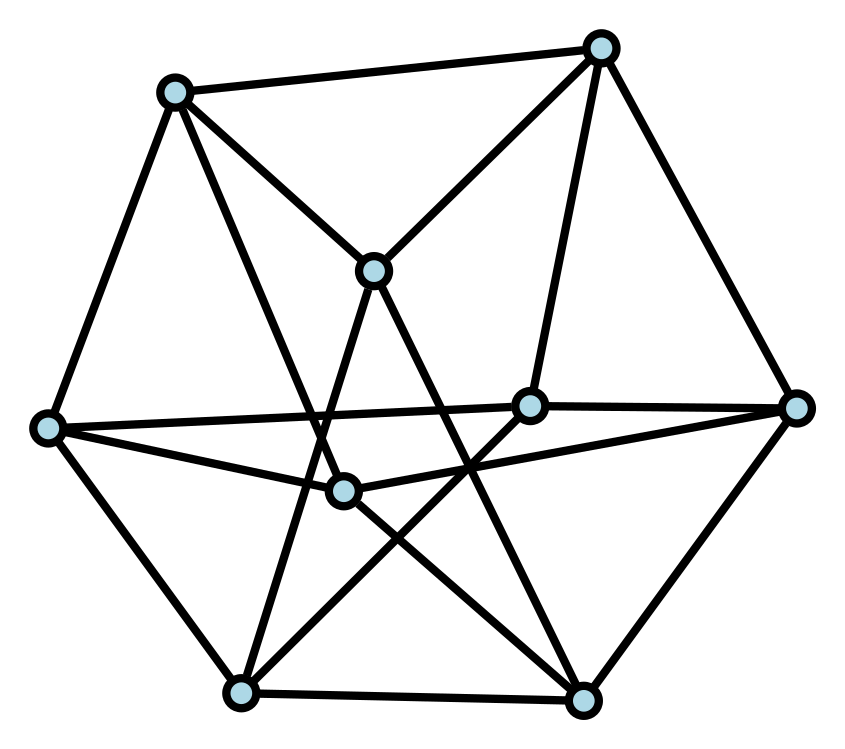
\includegraphics[width=8cm]{graph.png}
\end{center}

\end{frame}

\begin{frame}\frametitle{有向グラフの例}

\begin{center}
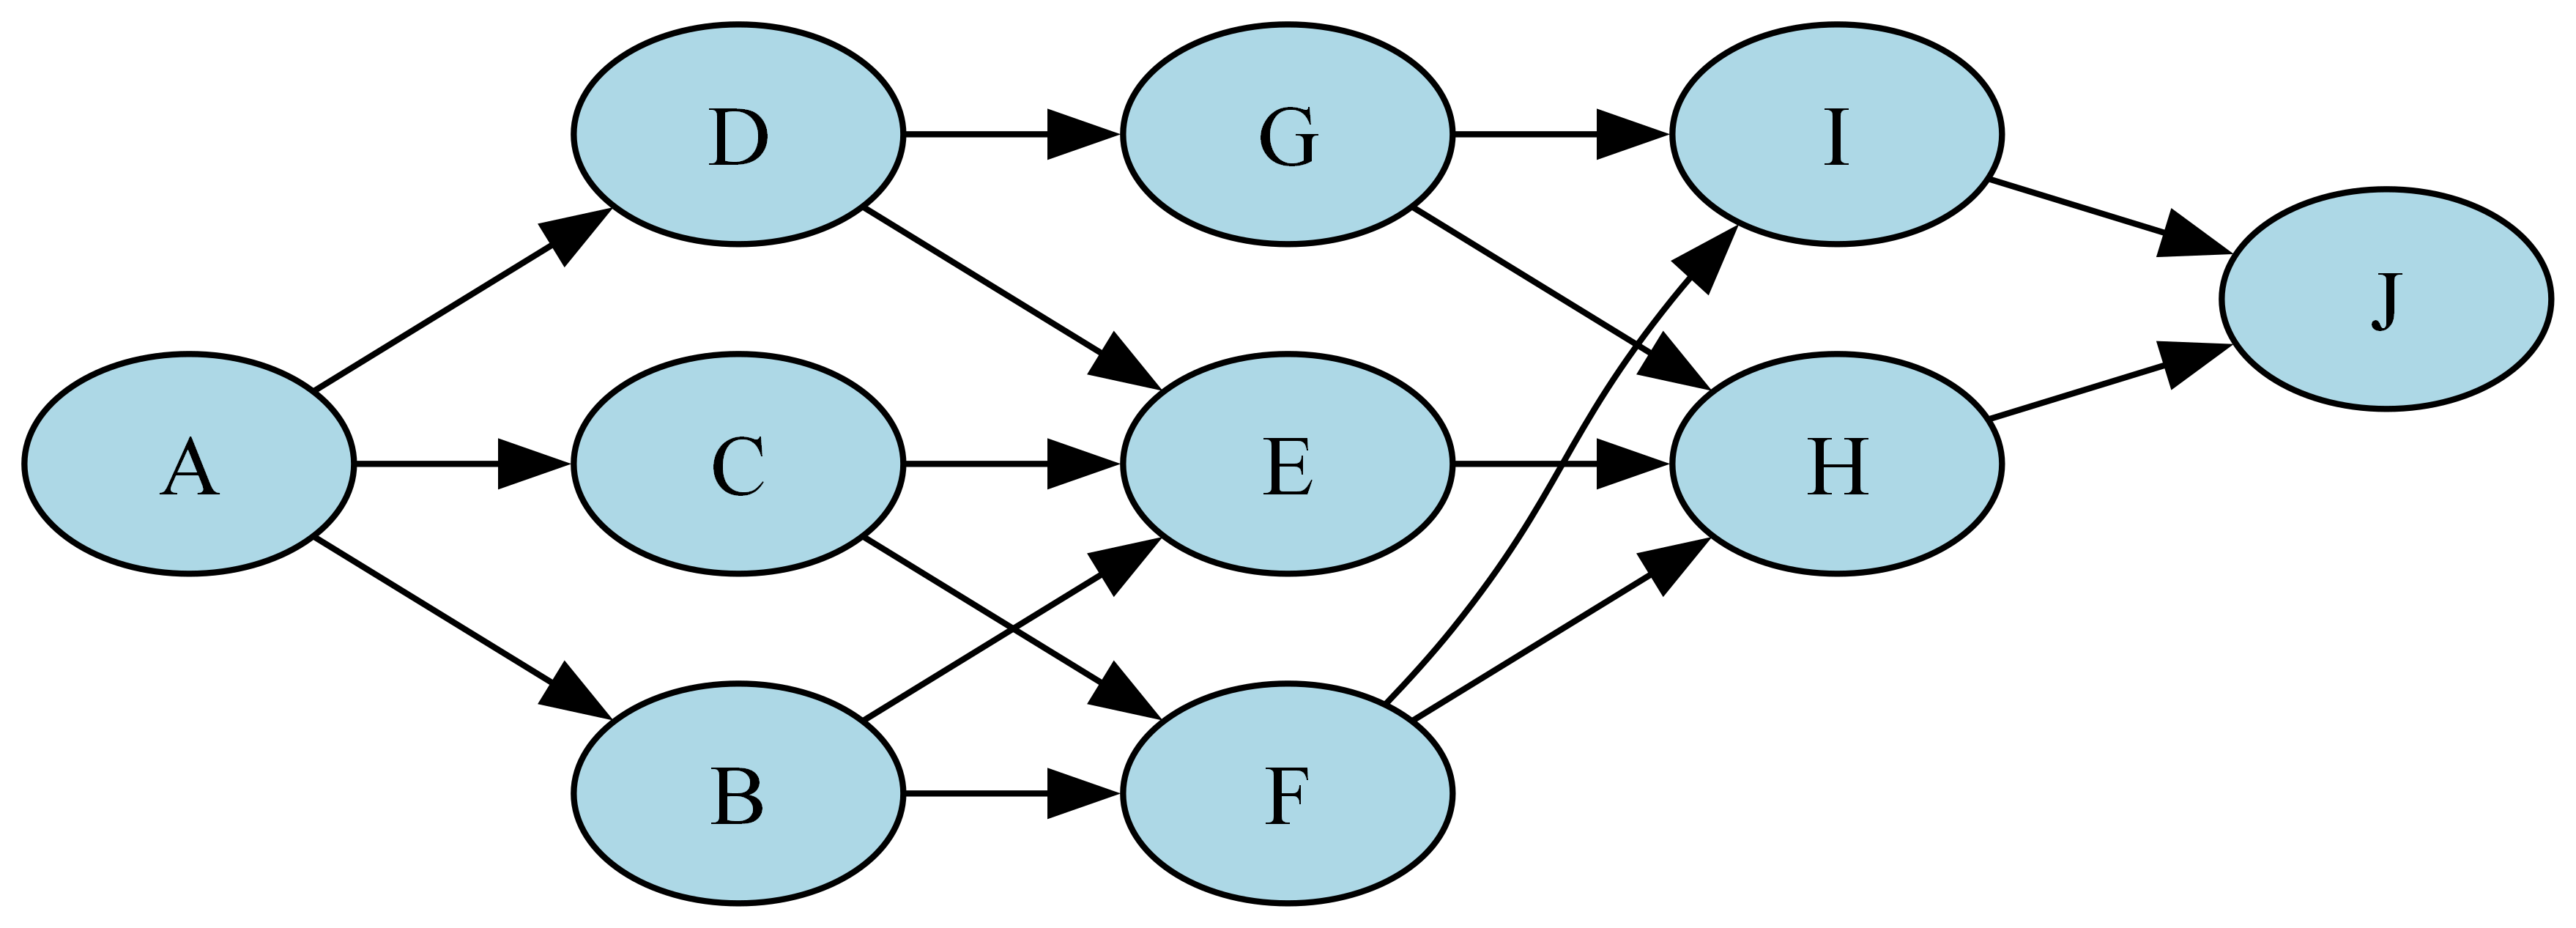
\includegraphics[width=15cm]{dag_example.png}
\end{center}

\end{frame}

\begin{frame}\frametitle{有向グラフの例おかわり}

\begin{center}
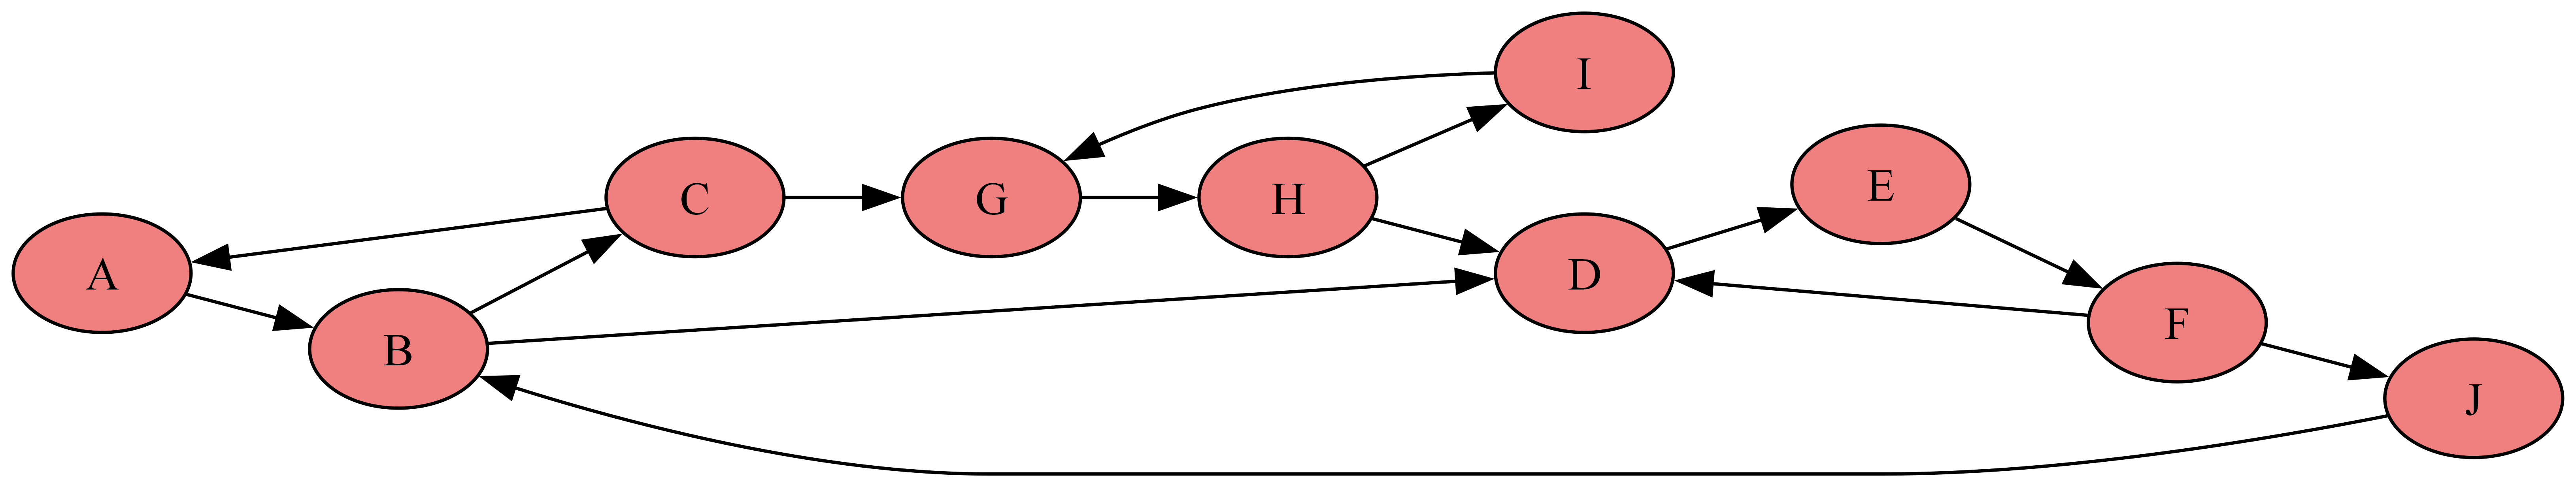
\includegraphics[width=15cm]{non_dag_example.png}
\end{center}

\end{frame}

\begin{frame}\frametitle{つまり…どういうことだってばよ?}

\begin{center}
\Huge{…で、その\structure{グラフ}は当社で働くうえで \\ 何のメリットがあるとお考えですか?}
\end{center}

\end{frame}

\begin{frame}\frametitle{来いよベネット!定義なんか捨ててかかって来い!}

\begin{block}{忙しい人向けのグラフ}
\begin{itemize}
\item グラフとは、「もの」とその「関係」を数学的にモデル化したものである
\item 「もの」は人間、駅、タスク、サーバなど
\item 「関係」は人間関係、線路、依存関係、ネットワークなど
\end{itemize}
\end{block}

\end{frame}

\begin{frame}\frametitle{トポロジカルソートって、何?}

\begin{definition}[二項関係]
集合$A$の直積$A\times A$の部分集合$R$を\structure{二項関係}と呼ぶ。 \\
また、$(a, b) \in R$を$aRb$と表す。
\end{definition}

\begin{definition}[半順序関係]
以下の性質を満たす関係$R$を\structure{半順序関係}と呼ぶ。
\begin{description}
\item[反射律] $\forall a \in A$に対して、$aRa$である
\item[反対称律] $a, b \in A$に対して、$aRb$かつ$bRa$ならば$a=b$である
\item[推移律] $a, b, c \in A$に対して、$aRb$ かつ $bRc$ならば$aRc$である
\end{description}
\end{definition}

\end{frame}

\begin{frame}\frametitle{トポロジカルソートって、何?}

\begin{definition}[線型順序]
集合$A$の半順序関係$R$において、$\forall a, b \in A$に対して$aRb$または$bRa$が成り立つならば、$R$は\structure{線型順序}であると呼ぶ。
\end{definition}

\begin{definition}[トポロジカルソート]
有向グラフ$G=(V, E)$の\structure{トポロジカルソート}とは、$V$の線型順序$(V, \leq)$で、$(u, v) \in E$ならば$u \leq v$を満たすものである。
\end{definition}

\end{frame}

\begin{frame}\frametitle{つまり…どういうことだってばよ?(2回目)}

\begin{center}
\Huge{…で、その\structure{トポロジカルソート}は(ry}
\end{center}

\end{frame}

\begin{frame}\frametitle{来いよベネット!定義なんか捨てて(ry}

\begin{block}{忙しい人向けのトポロジカルソート}
\begin{itemize}
\item 半順序関係は、大小関係や包含関係を抽象化したもの
\item 線型順序は、どれでも比較できるやつ、ぐらいの理解で
\item トポロジカルソートは、有向グラフの頂点をいい感じに順序付けしたもの
\end{itemize}
\end{block}

\end{frame}


\end{document}